\section{Optimizing the \FJ Plan}

\label{sec:optimization}

In the previous section we have introduced \FJ plans and their associated
data structures, the \GHTs.  We have seen that a \FJ plan is capable
of covering the entire design space in Fig.~\ref{fig:design-space},
from traditional join plans to \GJ.  In this section we describe how
to build, optimize, and speedup the execution of a \FJ plan.  We start
from a conventional binary plan produced by a query optimizer, and convert
it into an optimized \FJ plan (Section~\ref{sec:bj-to-fj}). Next, we
introduce the \COLT data structure to greatly reduce the cost of
building the hash tries (Section~\ref{sec:colt}).  We present a simple
vectorized execution algorithm for \FJ
(Section~\ref{sec:vectorized-execution}), and finally, we discuss how
\FJ relates to \GJ (Section~\ref{sec:fj-gj-multijoin}).

%%% In the previous section we have described how \FJ can simulate either binary
%%% join or \GJ, by simulating their data structures, query plans, and execution
%%% algorithms.  This allows \FJ to match the performance of either binary join or
%%% \GJ, if we simply instantiate \FJ to be the same as either algorithm. In this
%%% section we describe three key techniques that improve \FJ's performance
%%% beyond that of binary join and \GJ. First, we describe how to convert a binary
%%% plan into an efficient \FJ plan (Section~\ref{sec:bj-to-fj}). Next, we
%%% introduce the \COLT data structure to greatly reduce the cost of building
%%% the hash tries (Section~\ref{sec:colt}).  Then we present a simple
%%% vectorized execution algorithm for \FJ that improves cache locality
%%% (Section~\ref{sec:vectorized-execution}).  Finally, we conclude this section
%%% by discussing how \FJ relates to \GJ and other multiway join algorithms (Section~\ref{sec:fj-gj-multijoin}).

\subsection{Building and Optimizing a \FJ Plan}\label{sec:bj-to-fj}

Our system starts from an optimized binary plan produced by a
traditional cost-based optimizer; in particular, we use DuckDB's
optimizer~\cite{DBLP:conf/cidr/RaasveldtM20,DBLP:conf/vldb/Raasveldt22}. We
decompose a bushy plan into a set of left-deep plans, as described in
Sec.~\ref{sec:background}, then convert each left-deep plan into an
equivalent \FJ plan.  Finally, we optimize the converted \FJ plan,
resulting in a plan that can be anywhere between a left-deep plan or a
\GJ plan.

% fn gj2fj(gj_plan):
%   fj_plan = []
%   for x in gj_plan:
%     node = { r(x) | r $\in$ relations, x $\in$ r.schema }
%     fj_plan.push(node)
%   return fj_plan

\begin{figure}
  \begin{lstlisting}
fn binary2fj(bin_plan):
  fj_plan = []; r = bin_plan[0]
  $\phi_0$ = [ r(r.schema) ]; $\phi$ = $\phi_0$ # iterate over left relation
  for s in bin_plan[1:]:
    $\phi$.push(s(s.schema $\cap$ $avs(\phi)$)) # probe w/ available vars
    fj_plan.push($\phi$)
    $\phi$ = [ s(s.schema - $avs(\phi)$) ] # iterate over probe result
  fj_plan.push($\phi$)
  return fj_plan
\end{lstlisting}
  \caption{Translating a binary plans to a \FJ plan.}
  \label{fig:bj2fj}
\end{figure}

The conversion from a binary plan to an equivalent \FJ plan is done by the function
\lstinline|binary2fj| in Figure~\ref{fig:bj2fj}.  We begin by adding the full atom of the left
relation as the first subatom in the first \FJ plan node.  Then we iterate over
the remaining relations in the binary join plan.  For each relation, we add a
subatom whose variables are the intersection of the relation's schema with the
available variables at the current \FJ plan node. Then we create a new join
node, adding to it the relation with the remaining variables.

\begin{example}
  The binary plan $[R, S, T]$ for the clover query $Q_\clubsuit$ is
  converted into the \FJ plan shown in Eq.~\eqref{eq:bj-plan}.  For
  another example, consider a chain query:
  $$Q \cd R(x, y), S(y, z), T(z, u), W(u, v).$$
  The left-deep plan $[R, S, T, W]$ is converted into:
  $$[[R(x, y), S(y)], [S(z), T(z)], [T(u), W(u)], [W(v)]]$$
\end{example}

So far the algorithm in Figure~\ref{fig:bj2fj} produces a \FJ plan
that is equivalent to the left-deep plan.  Next, we
optimize the \FJ plan. The main idea behind our optimization is to
bring the query plan closer to \GJ, without sacrificing the benefits
of binary join.

For intuition, let us revisit the clover query $Q_\clubsuit$, and its
execution depicted in Fig.~\ref{fig:bj-loop} (as explained in
Example~\ref{ex:binary-free-join}).  Consider the input shown in
Fig.~\ref{fig:clover-vis}.  Both relations $R$ and $S$ are skewed on
the value $x_2$, and their join will produce $n^2$ tuples, namely
$\setof{(x_2, a_i, b_j)}{i, j \in [1..n]}$.  This means the body of
the second loop in Figure~\ref{fig:bj-loop} is executed $n^2$ times.
However, the $n^2$ tuples are only to be discarded by the join with
$T$ which does not contain $x_2$.

There is a simple fix to the inefficiency: we can pull the underlined
lookup on $T$ in Figure~\ref{fig:bj-loop} out of the loop over $s$ to
filter out redundant tuples early.  This results in the nested loops
in Figure~\ref{fig:factorized-loop} which runs in $O(n)$ time, because
the two lookups in the first loop already filter the result to a
single tuple.  At the logical level, we convert the first \FJ plan
into the second \FJ plan:
%
\begin{align*}
   & \mbox{Naive plan (Eq.~\eqref{eq:bj-plan}):} &  & [[R(x, a), S(x)], [S(b), T(x)], [T(c)]] \\
   & \mbox{Optimized plan:}                      &  & [[R(x, a), S(x), T(x)], [S(b)], [T(c)]]
\end{align*}
%
While this is closer to the \GJ in Figure~\ref{fig:gj-loop}, it
differs in that it still uses the same \GHTs built for original
plan, without the need for an additional hash table for $R$.

\begin{figure}
  \begin{lstlisting}
fn factor(plan):
  @outer: for i in [1..n-1].reverse():
    $\phi$ = plan[i]; $\phi'$ = plan[i-1]
    for $\alpha$ in $\phi$:
      if $\alpha$.vars $\subseteq avs(\phi) \wedge \alpha$.relation $\notin \phi':$
        $\phi$.remove($\alpha$); $\phi'$.push($\alpha$)
      else: continue @outer
\end{lstlisting}
  \caption{Factorizing a \FJ plan.}
  \label{fig:factorize-plan}
\end{figure}

More generally, we will optimize a \FJ plan by \emph{factoring out}
lookups, i.e. by moving a subatom from a node $\Phi_i$ to the node
$\Phi_{i-1}$.  In doing so we must ensure that the plan is still
valid, and also avoid accidental slowdowns.  For example, we cannot
factor the lookups on $S$ and $T$ beyond the outermost loop, because
that loop binds the variable $x$ used in the lookups.

The optimization algorithm for \FJ plans is shown in
Figure~\ref{fig:factorize-plan}. We traverse the plan in reverse order
visiting each node. For each node, if there is an atom whose variables
are all available before that node, and if the previous node does not
contain an atom of the same relation, we move the atom to the previous
node. These two checks ensure the factored plan remains valid.  The
last line in the algorithm ensures we factor lookups
\emph{conservatively}. That is, we factor out a lookup only if all
previous lookups in the same node have also been factored out. Doing
so respects the lookup ordering given by the original cost-based
optimizer, since scrambling this ordering may inadvertently slow down
the query. It should be clear that, except for extreme cases where the
enclosing loop is empty, factoring out any lookup will always improve
performance.


%%%%%  the ideas in this example are already included earlier, so I
%%%%%  commented it out
%%% \begin{example}
%%%   Given the \FJ plan in Eq.~\eqref{eq:bj-plan},
%%%   the algorithm in Figure~\ref{fig:factorize-plan} returns the plan 
%%%   $[[R(x, a), S(x), T(x)], [S(b)], [T(c)]]$. 
%%%   Figure~\ref{fig:bj-loop} shows the execution of the original plan, 
%%%   and Figure~\ref{fig:factorized-loop} shows the execution of the optimized plan.
%%% \end{example}


% \subsection{\COLT: Column-Oriented Lazy Trie}\label{sec:colt}

% The original \GJ algorithm builds a hash trie for each input relation.
% A left-deep plan avoids building a hash table on the left most
% relation, since it only needs to iterate over it, and this is an
% important optimization, since the left most relation is often the
% largest one.  Building a subtrie can also be wasteful when that
% subtrie's parent is pruned away by an earlier join, in which case the
% subtrie will never be used.  To address that, we describe here how to
% build the tries \emph{lazily}: we only build the trie for a
% (sub-)relation at runtime, if and when we need to perform a lookup, or
% need to iterate over a prefix of its tuples.  This idea leads to our
% new data structure called Column-Oriented Lazy Trie, or \COLT for
% short.  In our system  the raw data is stored column-wise, in main
% memory, and each column is stored as a vector, as standard in
% column-oriented databases~\cite{DBLP:journals/ftdb/AbadiBHIM13}.
% %
% \begin{definition}
%   A \emph{\COLT} is a tree where each leaf is a vector of offsets into
%   the base relation, and each internal node is a hash map mapping a
%   tuple to a child node.
% \end{definition}


% \begin{figure}
%   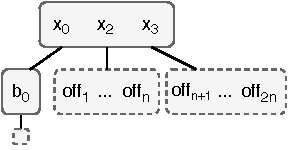
\includegraphics[width=0.3\linewidth]{colt.pdf}
%   \caption{A \COLT for the relation $S$ in
%     Fig.~\ref{fig:clover-query}. Each off$_i$ is an integer
%     representing an offset into the table $S$.}
%   \label{fig:colt}
% \end{figure}

% A \COLT tree need not be balanced, and there can be both hash maps and
% vectors at the same tree level.  Fig.~\ref{fig:colt}
% illustrates a \COLT tree for the instance $S$ of the clover query
% $Q_\clubsuit$.

% %%% \begin{example}\label{ex:colt}
% %%%   Recall the relation $S$ for the clover query $Q_\clubsuit$, 
% %%%   whose \GHTs are shown in Figure~\ref{fig:ght-examples}.
% %%%   Figure~\ref{fig:colt} shows a \COLT for $S$.
% %%% \end{example}


% \begin{figure}
%   \begin{lstlisting}
% struct COLT {
%   relation, schema, vars, 
%   data = Map(HashMap<Tuple, COLT>) | Vec<Vec<u64>> }

% impl GHT for COLT:
%   fn new(relation, schema):
%     COLT { relation, schema, schema[0],
%            data = [ 0, 1, ..., relation.len - 1 ] }

%   fn iter():
%     match self.data:
%       Map(m) => m.keys().iter(),
%       Vec(v) => 
%           if is_suffix(self.vars, relation.schema):
%             v.map(|i| cols = self.relation[self.vars];
%                       cols.map(|c| c[i]) )
%           else: self.force(); self.iter()

%   fn get(key): self.force(); self.get_map.get(key)

%   fn force():
%     match self.data:
%       Map(m) => {} # already forced, do nothing
%       Vec(v) => 
%         map = new()
%         for i in v:
%           cols = self.relation[self.vars]
%           k = cols.map(|col| col[i])
%           if map[k] is None: # make a new, empty COLT
%             map[k] = COLT { relation: self.relation, 
%                             schema: self.schema[1..], 
%                             data: [] }
%           map[k].data.push(i)
%         self.data = Map(map)
% \end{lstlisting}
%   \caption{The \COLT data structure.}
%   \label{fig:colt-impl}
% \end{figure}

% % \ds{I did not understand the rest of this section.  What is needed:
% %   (a) explain how the raw data is stored.  For example, how is a
% %   relation $R(x,y,z)$ stored: row-wise? column-wise? sorted? (b) where
% %   are the indices pointing to?  For example, if I construct the first
% %   level of $R(x,y,z)$, then for each value of $x$ I have a set of
% %   indices: where are these indices pointing to?}
% % \rw{I added an example to explain this.}

% \COLT Implements the \GHT interface in Figure~\ref{fig:ght}, and its
% implementation is shown in Figure~\ref{fig:colt-impl}. As before,
% \COLT stores a reference to the relation it represents, as well as the
% \GHT schema computed from the plan.
% %%% Recall the $i$-th element of the schema contains the variables at
% %%% the $i$-th level of the trie.  For a (sub-)\COLT at level $k$,
% %%% \lstinline|vars| is the same as the $k$-th element of the
% %%% schema. the $0$-th element of the schema.
% Consider a relation with $n$ tuples.  The \COLT tree is initialized
% with a single node consisting of the vector $[0, \ldots, n-1]$,
% i.e. one offset to each tuple.  
% \COLT
% implements the \lstinline|get| and \lstinline|iter| methods lazily.  
% When
% \lstinline|get| is called, we check if the current node is a hash
% map or a vector.  In the first case, we simply perform a lookup in the
% map.  In the second case, we first replace the current vector with a
% hash map, whose children are vectors of offsets.  Notice that this
% requires iterating over the current vector of offsets, accessing the
% tuple in the base table, inserting the key in the hash map, and
% inserting the offset in the corresponding child.  Consider now a call
% to \lstinline|iter|.  If the current node is a hash map, then we
% return an iterator over it.  If it is a vector, then we check if it is
% a suffix of the relation schema: if yes, then we simply iterate over
% that vector (and access the tuples via their offsets), otherwise we
% first materialize the current hash map as explained above, and return
% an iterator over the hash map.

% As a simple but effective optimization, we do not initialize the \COLT
% tree to the single node $[0,1,\ldots,n-1]$, but instead iterate
% directly over the base table, if required.  If no \lstinline|get|
% is performed on this table, then we have completely eliminated the
% cost of building any auxiliary structure on this table.  Thus, the \FJ
% plan can be equivalent to a left-deep plan that avoids building a hash
% table on the left-most relation.  \COLT is also closer to the structure of
% traditional hash tables, which, in some implementations, map a key to
% a vector of pointers to tuples.
% %
% %%% Note that the \COLT for each relation of size $n$ is always initialized to be the 
% %%%   vector $[0, \ldots, n-1]$.
% %%% Since we can only iterate over this vector, 
% %%%   we did not have to materialize it in the first place.
% %%% Instead, we can simply loop over the tuples in the original relation 
% %%%   when \lstinline|iter| is called.
% %%% This means when the \FJ plan is equivalent to a binary plan, 
% %%%   we completely eliminate the cost of trie building for the left relation, 
% %%%   recovering the behavior of binary join.
% %
% %%% \COLT also captures the structure of hash tables more closely than
% %%% \GHTs.  Recall that a hash table maps each key to an entire tuple in
% %%% the relation.  Equivalently, we can also map the key to the row index
% %%% of the tuple.  But that is precisely a \COLT whose first level is
% %%% materialized.

% \begin{example}\label{ex:colt-clover}
% Consider an extension of the clover query $Q_\clubsuit$:
% \begin{align*}
%   Q(x, a, b, c) \cd R(x,a), S(x,b), T(x, c), \underline{U(b)}.
% \end{align*}
%   % 
% %   \begin{lstlisting}[
% %     language=SQL,
% %     showspaces=false,
% %     basicstyle=\ttfamily\small,
% %     commentstyle=\color{gray},
% %     escapeinside={(*}{*)},
% %  ]
% % SELECT * FROM R,S,T,U -- schema: R(x,a),S(x,b),T(x,c),U(b)
% %  WHERE R.x = S.x AND S.x = T.x AND T.x = R.x AND (*\underline{S.b = U.b}*)
% % \end{lstlisting}
% %
% \GJ builds a 2-level hash trie for each of $R$, $S$, and $T$, as well
% as a 1-level hash trie for $U$.  Consider the \FJ plan
% $[[R(x,a),S(x),T(x)],[U(b),S(b)],[T(c)]]$.  \FJ executes the first
% node of the plan by iterating over $R$ directly, without constructing
% any auxiliary structure. For each tuple $(x, a)$ in $R$, it looks up
% $x$ in $S$ and $T$.  Upon the first lookup, \COLT builds the first
% level of the \GHT for $S$ and $T$, i.e. a hash map indexed by the $x$
% values.  Assuming the database instance for $R,S,T$ shown in
% Fig.~\ref{fig:clover-query}, the result of $R.x \cap S.x \cap T.x$ has
% only one value, $x_0$, thus, $\FJ$ executes the second node for only
% one value $x_0$.  Here it needs to intersect $U(b)$ and $S(b)$.
% Assume for the moment that \FJ chooses $U(b)$ to be the cover, on the
% first lookup in $S$, \COLT will expand the second level, arriving at
% Figure~\ref{fig:colt}: notice that all other $b$ values in $S$ will
% never be inserted in the hash table.  More realistically, \FJ follows
% the principle in \GJ and chooses $S(b)$ as cover, because it is the
% smallest: it builds a hash map for $U$, but none for the 2nd level of
% $S$.
% \end{example}

% The example highlights a divergence between \GJ and traditional plans.
% To intersect $R_1.x \cap R_2.x \cap \ldots$, \GJ choose to iterate
% over the smallest relation, which results in the best runtime {\em
%   ignoring} the build time.  A traditional join plan will iterate over
% the largest relation, because then it needs to build hash tables only
% on the smaller relations.  Currently, we follow \GJ, and plan to
% explore alternatives in the future.

% % \ds{Remy please check the example and the discussion}


% % \ds{The example doesn't help.  Once we have identified the single
% %   value $b_0$, we only need to look it up in $U(b)$.  But since we
% %   haven't constructed anything for $U$ yet, this requires a full scan
% %   of $U$.  This is modestly better than scanning $U$ to create a
% %   hash-table, but I don't see how this savings generalizes.  If the
% %   previous joins return the values $b_0, b_1, b_2, \ldots$, then how
% %   can we look them up in $U$ more efficiently than computing a hash
% %   table on $U$?}
% % \rw{Scanning $U$ while probing into the small trie is much faster than 
% % building a hash table for $U$, since the latter needs to allocate memory.
% % But the main point is not about $U$, but rather we avoid building a large 
% % part of the second level of $S$.  }

% \subsection{Vectorized Execution}\label{sec:vectorized-execution}
% The \FJ algorithm as presented in Figure~\ref{fig:fj-algo}
%   suffers from poor temporal locality.
% In the body of the outer loop, 
%   we probe into the same set of relations for each tuple.
% However, these probes are interrupted by the recursive 
%   call at the end, 
%   which is itself a loop interrupted by further recursive calls.

% \begin{figure}
%   \begin{lstlisting}
% @outer for ts in tries[0].iter_batch(batch_size):
%   tup_subtries = [(tuple + t, [ tries[0].get(t) ]) | t $\in$ ts]
%   for trie in tries[1..]:
%     for (tup, subtries) in tup_subtries:
%       subtrie = trie.lookup(tup[trie.vars])
%       if subtrie is None:
%         tup_subtries.remove((tup, subtries))
%       else: subtries.append(subtrie)
%   for (tup, subtries) in tup_subtries:
%     new_tries = all_tries[tries $\mapsto$ subtries]
%     join(new_tries, plan[1:], tup)
% \end{lstlisting}
%   \caption{Vectorized execution for \FJ.}
%   \label{fig:vectorized-execution}
% \end{figure}

% A simple way to improve locality is to perform a batch of probes 
%   before recursing, just like the classic vectorized execution 
%   for binary join.
% Concretely, we replace the \lstinline|iter| method 
%   with a new method \lstinline|iter_batch(batch_size)|
%   which returns up to \lstinline|batch_size| tuples at a time.
% If there are less than \lstinline|batch_size| tuples left, 
%   it returns all the remaining tuples.
% Then we replace the outer loop in Figure~\ref{fig:fj-algo} 
%   with the one in Figure~\ref{fig:vectorized-execution}.
% For each batch of tuples, 
%   we create a vector pairing each tuple to its subtrie in 
%   \lstinline|tries[0]|.
% Then for each trie to be probed,
%   we iterate over the vector and look up each tuple 
%   from the trie.
% If the lookup succeeds, we append the subtrie to the vector of tries paired with the tuple.
% If it fails, we remove the tuple to avoid probing it again.
% Finally, with each tuple and the subtries it pairs with, 
%   we recursively call \lstinline|join|.

% \subsection{Discussion}\label{sec:fj-gj-multijoin}

% \COLT is a lazy data structure, sharing a similar goal with database
% cracking~\cite{DBLP:conf/cidr/IdreosKM07,DBLP:conf/sigmod/IdreosKM07}, where an
% index is constructed incrementally, by performing a little work during each
% lookup. 
% % \rw{Dan, can you check the following?}
% Another connection is to Factorized Databases~\cite{DBLP:journals/sigmod/OlteanuS16} -- we
% intentionally used the term ``factor'' when describing how we optimize \FJ plans to
% suggest this connection. 
% Concretely, we can view the trie data structure as a
% factorized representation of a relation, where keys of the same hash map are
% combined with union, and tuples are formed by taking the product of values at
% different levels. Practically, we can use this factorized representation to 
% compress large outputs, saving time and space during materialization.

% As we discussed at the end of Section~\ref{sec:free-join}, in order
% match the optimality of \GJ, the \FJ algorithm needs to choose
% dynamically the ``cover'', i.e. the relation over which to iterate.  To
% achieve this, we first find {\em all} covers for each node, then make a simple
% change to the \FJ algorithm in Figure~\ref{fig:fj-algo}: we simply
% choose to iterate over the cover whose trie has the fewest keys.  For
% that we insert the following code right before the outer loop in
% Figure~\ref{fig:fj-algo}:
% %
% \begin{lstlisting}
% trie[0] = covers(plan[0]).min_by(|t| t.keys().len)
% trie[1..] = # the rest of the tries
% \end{lstlisting}
% %
% When we use \COLTs, we cannot know the exact number of keys in a vector unless
%   we force it into a hash map. In that case we use the length of the vector as
%   an estimate.

% \begin{example}
%   Consider the triangle query $Q_\triangle$, and the following \FJ plan:
%   $$[[R(x), T(x)], [R(y), S(y)], [S(z), T(z)]]$$  Each subatom is a
%   cover of its own node.  On the outermost loop, we iterate over $R$
%   if it has fewer $x$ values, and otherwise we iterate over $T$.  On
%   the second loop level we make a decision picking between $S$ and a
%   subtrie of $R$, \emph{for each subtrie of $R$}.  Finally, on the
%   innermost loop we pick between the subtries of $S$ and $T$.
% \end{example}

% % \ds{I recommend removing the paragraph below}
% % Another small tweak allows \FJ to further capture other classic
% % multiway joins. Just like how \GJ dynamically choose the relation to iterate
% % over, various classic multiway joins, such as Hash Team~\cite{} and Eddies~\cite{},
% %  also dynamically orders the relations to
% % probe into. We support this by inserting another line right before the 
% % inner loop of Figure~\ref{fig:fj-algo}:
% % %
% % \begin{lstlisting}
% % tries[1..].sort_by(probe_cost)
% % \end{lstlisting}
% % %
% % Here \lstinline|probe_cost| estimates the cost of probing into each trie.
% % The simplest cost function returns the size of the trie;
% % a more advanced one may perform some form of selectivity estimation;
% % and a sophisticated cost model can even receive feedback from previous 
% % iterations of the loop.